%% ----------------------------------------------------------------
%% Thesis.tex -- MAIN FILE (the one that you compile with LaTeX)
%% ---------------------------------------------------------------- 

% Set up the document
\documentclass[a4paper, 11pt, oneside]{Thesis}  % Use the "Thesis" style, based on the ECS Thesis style by Steve Gunn
\graphicspath{Figures/}  % Location of the graphics files (set up for graphics to be in PDF format)

% Include any extra LaTeX packages required
\usepackage{graphicx}
\usepackage[square, numbers, comma, sort&compress]{natbib}  % Use the "Natbib" style for the references in the Bibliography
\usepackage{verbatim}  % Needed for the "comment" environment to make LaTeX comments
\usepackage{vector}  % Allows "\bvec{}" and "\buvec{}" for "blackboard" style bold vectors in maths
\hypersetup{urlcolor=blue, colorlinks=true}  % Colours hyperlinks in blue, but this can be distracting if there are many links.

%% ----------------------------------------------------------------
\begin{document}
\frontmatter      % Begin Roman style (i, ii, iii, iv...) page numbering

% Set up the Title Page
\title  {Virtual Arduino}
\authors  {\texorpdfstring
            {\href{your web site or email address}{Ebtessam Zoheir}}
            {Ebtessam Zoheir}
            }
            
\title  {Virtual Arduino}
           
\addresses  {\groupname\\\deptname\\\univname}  % Do not change this here, instead these must be set in the "Thesis.cls" file, please look through it instead

\supervisor  {\texorpdfstring
            {\href{http://met.guc.edu.eg/People/Profile.aspx?facId=2998}{Georg Jung}}
            {Georg Jung}
            }  
\date       {\today}
\subject    {}
\keywords   {}

\maketitle
%% ----------------------------------------------------------------

\setstretch{1.3}  % It is better to have smaller font and larger line spacing than the other way round

% Define the page headers using the FancyHdr package and set up for one-sided printing
\fancyhead{}  % Clears all page headers and footers
\rhead{\thepage}  % Sets the right side header to show the page number
\lhead{}  % Clears the left side page header

\pagestyle{fancy}  % Finally, use the "fancy" page style to implement the FancyHdr headers

%% ----------------------------------------------------------------
% Declaration Page required for the Thesis, your institution may give you a different text to place here
\Declaration{

\addtocontents{toc}{\vspace{1em}}  % Add a gap in the Contents, for aesthetics

I, Ebtessam Zoheir, declare that this thesis titled, `Virtual Arduino' and the work presented in it are my own. I confirm that:

\begin{itemize} 
\item[\tiny{$\blacksquare$}] This work was done wholly or mainly while in candidature for a research degree at this University.
 
\item[\tiny{$\blacksquare$}] Where any part of this thesis has previously been submitted for a degree or any other qualification at this University or any other institution, this has been clearly stated.
 
\item[\tiny{$\blacksquare$}] Where I have consulted the published work of others, this is always clearly attributed.
 
\item[\tiny{$\blacksquare$}] Where I have quoted from the work of others, the source is always given. With the exception of such quotations, this thesis is entirely my own work.
 
\item[\tiny{$\blacksquare$}] I have acknowledged all main sources of help.
 
\item[\tiny{$\blacksquare$}] Where the thesis is based on work done by myself jointly with others, I have made clear exactly what was done by others and what I have contributed myself.
\\
\end{itemize}
 
 
Signed:\\
\rule[1em]{25em}{0.5pt}  % This prints a line for the signature
 
Date:\\
\rule[1em]{25em}{0.5pt}  % This prints a line to write the date
}
\clearpage  % Declaration ended, now start a new page

%% ----------------------------------------------------------------
% The "Funny Quote Page"
%\pagestyle{empty}  % No headers or footers for the following pages

%\null\vfill
% Now comes the "Funny Quote", written in italics
%\textit{``Write a funny quote here.''}

%\begin{flushright}
%If the quote is taken from someone, their name goes here
%\end{flushright}

%\vfill\vfill\vfill\vfill\vfill\vfill\null
%\clearpage  % Funny Quote page ended, start a new page
%% ----------------------------------------------------------------

% The Abstract Page
\addtotoc{Abstract}  % Add the "Abstract" page entry to the Contents
\abstract{
\addtocontents{toc}{\vspace{1em}}  % Add a gap in the Contents, for aesthetics

Virtual Arduino is a desktop application that simulates the Arduino board. It is an educational tool aims to provide hands-on experience for embedded systems programming and hardware beginners. This includes writing, verifying and uploading Arduino code. It should also include building hardware circuits to connect with the Arduino. The interactive simulator will help the user visualize the output of the code and the hardware failure scenarios make it more like real-life. These concepts give Virtual Arduino an edge over other simulators out there\ldots
 
}

\clearpage  % Abstract ended, start a new page
%% ----------------------------------------------------------------

\setstretch{1.3}  % Reset the line-spacing to 1.3 for body text (if it has changed)

% The Acknowledgements page, for thanking everyone
%\acknowledgements{
%\addtocontents{toc}{\vspace{1em}}  % Add a gap in the Contents, for aesthetics

%The acknowledgements and the people to thank go here, don't forget to %include your project advisor\ldots

%}
\clearpage  % End of the Acknowledgements
%% ----------------------------------------------------------------

\pagestyle{fancy}  %The page style headers have been "empty" all this time, now use the "fancy" headers as defined before to bring them back


%% ----------------------------------------------------------------
\tableofcontents  % Write out the Table of Contents

%% ----------------------------------------------------------------
%\lhead{\emph{List of Figures}}  % Set the left side page header to "List if Figures"
%\listoffigures  % Write out the List of Figures

%% ----------------------------------------------------------------
%\lhead{\emph{List of Tables}}  % Set the left side page header to "List of Tables"
%\listoftables  % Write out the List of Tables

%% ----------------------------------------------------------------
%\setstretch{1.5}  % Set the line spacing to 1.5, this makes the following tables easier to read
%\clearpage  % Start a new page
%\lhead{\emph{Abbreviations}}  % Set the left side page header to "Abbreviations"
%\listofsymbols{ll}  % Include a list of Abbreviations (a table of two columns)
%{
% \textbf{Acronym} & \textbf{W}hat (it) \textbf{S}tands \textbf{F}or \\
%\textbf{LAH} & \textbf{L}ist \textbf{A}bbreviations \textbf{H}ere \\

%}

%% ----------------------------------------------------------------
%\clearpage  % Start a new page
%\lhead{\emph{Physical Constants}}  % Set the left side page header to %"Physical Constants"
%\listofconstants{lrcl}  % Include a list of Physical Constants (a four %column table)
%{
% Constant Name & Symbol & = & Constant Value (with units) \\
%Speed of Light & $c$ & $=$ & $2.997\ 924\ 58\times10^{8}\ \mbox{ms}^{-\mbox{s}}$ (exact)\\

%}

%% ----------------------------------------------------------------
%\clearpage  %Start a new page
%\lhead{\emph{Symbols}}  % Set the left side page header to "Symbols"
%\listofnomenclature{lll}  % Include a list of Symbols (a three column table)
%{
% symbol & name & unit \\
%$a$ & distance & m \\
%$P$ & power & W (Js$^{-1}$) \\
%& & \\ % Gap to separate the Roman symbols from the Greek
%$\omega$ & angular frequency & rads$^{-1}$ \\
%}
%% ----------------------------------------------------------------
% End of the pre-able, contents and lists of things
% Begin the Dedication page

%\setstretch{1.3}  % Return the line spacing back to 1.3

%\pagestyle{empty}  % Page style needs to be empty for this page
%\dedicatory{For/Dedicated to/To my\ldots}

%\addtocontents{toc}{\vspace{2em}}  % Add a gap in the Contents, for aesthetics


%% ----------------------------------------------------------------
\mainmatter	  % Begin normal, numeric (1,2,3...) page numbering
\pagestyle{fancy}  % Return the page headers back to the "fancy" style

% Include the chapters of the thesis, as separate files
% Just uncomment the lines as you write the chapters

\lhead{\emph{Introduction}}  % Set the left side page header to "Introduction"

\chapter{Introduction}

The use of microcontroller evaluation boards is becoming more popular year by year. The post by Oskay, W. on \href{http://electronics.stackexchange.com/questions/2324/why-are-atmel-avrs-so-popular}{Why are Atmel AVRs so popular?} on April 22nd 2010 gives insight on the importance of Arduino and similar AVR based boards. The fact that the Arduino is easily programmed in C, has built-in Analog Digital Converter (ADC), Pulse Width Modulation (PWM) and has good cross-platform support makes it a very efficient way to learn and practice embedded system programming.

Given the importance of AVR microcontroller boards, acknowledging the fact that not all students have access to such evaluation boards we have decided that a simulator which could virtually replace the Arduino experience would be useful. Already existing simulators do not provide close to real life experience and hence cannot replace the actual Arudino. Differences between the Virtual Arduino project and already existing ones will be discussed later in the paper.

Our aim is to make a real time hardware simulator that is as close as possible to the real life experience. The simulator will later achieve this by covering all aspects of an embedded system including hardware components, hardware interfacing, hardware failure, board setting, code compiling and uploading and finally visualizing the whole process. Another advantage is that it will give the user a wider variety of hardware components to work with that may not be available or may be too expensive. The simulator library will be very flexible and easily scalable to include future components and newer versions of the boards.

\clearpage  % Introduction ended, start a new page
 % Introduction

\lhead{\emph{Background}}  % Set the left side page header to "Background"

\chapter{Background}

Arduino is an open-source electronics prototyping platform based on flexible, easy-to-use hardware and software, retrieved from \href{http://arduino.cc/en/}{Arduino.cc}. The Arduino board is designed around the 8-bit Atmel AVR microcontroller. Its software is composed of a standard C-based programming language compiler and a boot loader that executes on the microcontroller.



\section{Program Specs}

\begin{figure}[h!]
\centering
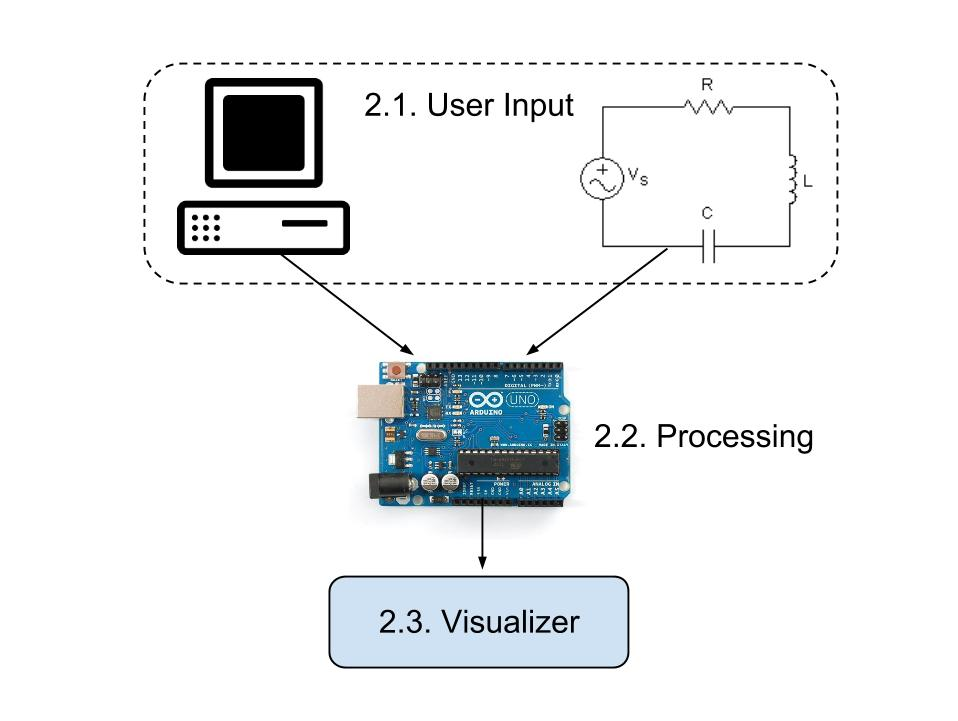
\includegraphics[height=9cm, width=12cm]{Hierarchy.jpg}
\caption{Virtual Arduino Architecture}
\label{Architecture}
\end{figure}
The following section will discuss the architectural hierarchy of the full program. The section will also partition the program into modules so it can be more easily conquered. 

\subsection{User Input}
The architecture is divided into three main parts, first part in the user input which can be in form  of text i.e Arduino code or in the form of circuitry.

\subsubsection{Computer Module}
Real-life Arduino system can be divided into two parts, Integrated development environment (IDE) and hardware. The IDE or Computer Module is where the user can write, compile and upload code onto the Arduino. This shall be implemented by using the already existing opensource Arduino IDE and redirecting its output to a virtual serial port so that this binary code can be later used for the simulation. This binary code will be transimitted down from user input to the processing module. Details about the computer mode internal workings shall be dicussed in sections 2.2 amd 2.3.

\subsubsection{Circuitry Module}
The second part of the Arduino experience is external hardware. One of the main advantages of the Arduino board is that it is easily interfaceable with most hardware components as it has built-in ADC and PWM. This module is where the user gets to experiment with hardware and connect with the Arduino board. The circuitry workspace should include an easily scalable hardware library and a circuit builder. The hardware components are divided into 3 types which are input, connectors and output. Input components are mainly sensors, connector components are wires and resistors and output components are LEDs and motors. We plan on implementing this part by using and already existing opensource simulator and upgrading its GUI and its hardware components to fit the concept of the Virtual Arduino. This will be done by adding some hardware failures scenarios and giving the simulator a more realistic GUI. The circuit output or simplification if I may say so will also be sent to the next level of the architecture for further processing and linking with Computer Module output. 

\subsection{Processing Module}
This module is the junction between the upper and lower level of the architecture. It takes the binary code from the Computer Module and translates it into actions in the Virtual Arduino processor. After evaluating the different internal components of the processor the Virtual Arduino output pins shall be assessed and this will reflect on the different output hardware components. The status of the different hardware components - whether high, low or PWM signal- shall be sent to the next level of the architecture which is the Visualizer.

\subsection{Visualizer}
This is the part where the user sees the output of his program. After the code is verified and is clear of any syntactic errors the user uploads the code onto his/her Virtual Arduino and output components start to show changes. The user will also be able to alter the environment by changing the input to the sensor and see the immediate change in the output components. 

\section{Bootloader}
\label{sec:bootloader}
\begin{figure}[h!]
\centering
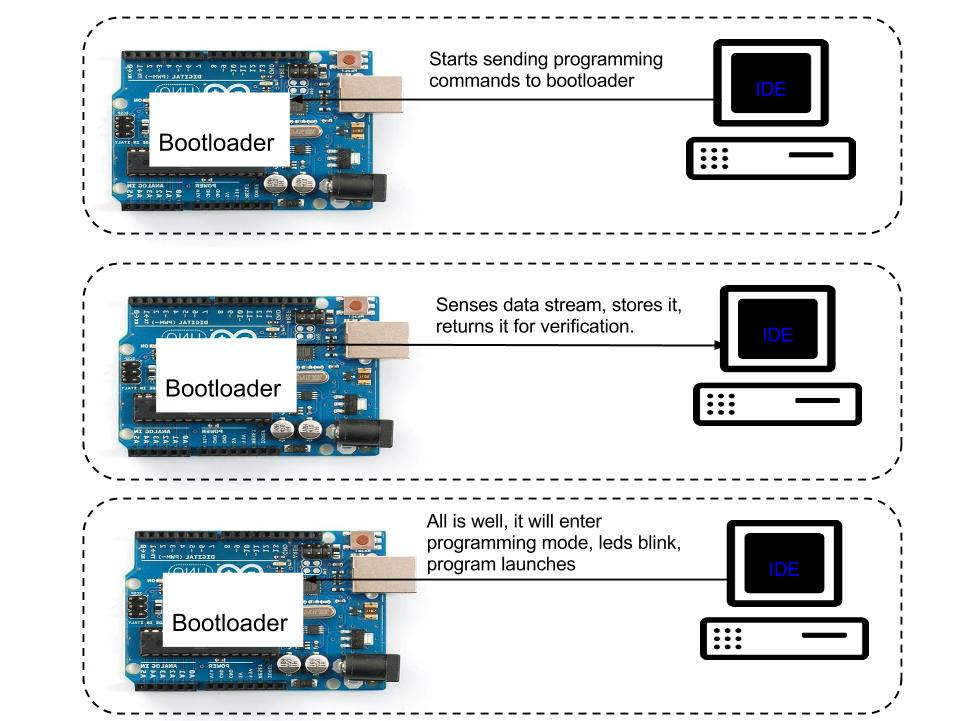
\includegraphics[height=9cm, width=12cm]{Bootloader.jpg}
\caption{Bootloader-Programmer Handshake}
\label{Bootloader Handshake}
\end{figure}
Stackoverflow \cite{Stackoverflow:URL} user \emph{angelatlarge} commented on April 3, 2013 (\href{http://stackoverflow.com/questions/15785087/upload-arduino-code-on-virtual-serial-port-through-arduino-ide/15792961?noredirect=1#comment22546153_15792961}{Upload Arduino code on virtual serial port through Arduino IDE}):
\begin{quotation}
``The process of uploading code is not a uni-directional process. There is a program on the Arduino called a bootloader [\emph{later discussed in section \ref{sec:bootloader}, the author}] which is responsible for communicating with the programmer (``programmer'': a program that programs the Arduino, assume it is the Arduino IDE for now). The Arduino CPUs cannot be programmed across serial lines. Rather these chips are programmed either via the \href{http://www.atmel.com/images/doc0943.pdf}{in system programming (ISP)} or via the \href{http://en.wikipedia.org/wiki/Jtag}{JTAG protocol}.
\end{quotation}
Retrieved from \href{http://stackoverflow.com/questions/15785087/upload-arduino-code-on-virtual-serial-port-through-arduino-ide/15792961?noredirect=1#comment22546153_15792961}{Stackoverflow}. 
Angelatlarge added  (2013, April 3).\href{http://stackoverflow.com/questions/15785087/upload-arduino-code-on-virtual-serial-port-through-arduino-ide/15792961?noredirect=1#comment22546153_15792961}{Upload Arduino code on virtual serial port through Arduino IDE} \begin{quotation}``The bootloader is a program that runs on the Arduino CPU, the program runs at startup and looks for programming commands over the serial port. If it discovers that a programmer is trying to communicate programming information, it will read the compiled Arduino binary coming over the serial link, store it in flash memory, send it back over the serial link for verification, and if everything is successful, exit and launch the stored sketch. If no programming information appears on the serial port, that is, no programmer is trying to write a new sketch, then the bootloader simply quits and launches the program already stored in flash.\end{quotation} Retrieved from http://stackoverflow.com/questions/15785087/upload-arduino-code-on-virtual-serial-port-through-arduino-ide/15792961?noredirect=1#comment22546153_15792961. 

Each Arduino board uses a different bootloader. In our program we will be simulating the ArduinoUno which uses the \href{https://github.com/arduino/Arduino/tree/master/hardware/arduino/bootloaders/optiboot}{optiboot bootloader} (publicly available on GitHub \cite{GitHub:URL}). Our plan is to mimic the responses sent from the bootloader to the IDE in order to get the code the is sent from the IDE to the flash on the Arduino board. The bootloader communicates with the IDE using the \href{http://www.atmel.com/Images/doc2525.pdf}{STK500 protocol}. The STK500 is a communication protocol of 8-bit AVR. The handshake in Figure 2.2 will also be discussed in further details in the next chapter.

\section{Communication}
In order to imitate the bootloader we had to sniff the serial port to understand what is being transmitted between the IDE and the board. First the Programmer in the IDE tries to sync with a device so it sends an GETSYNC command ([30] [20]) if a device is connected the bootloader on the device replies with INSYC, OK ([14] [10]). After establishing the connection the Programmer asks the bootloader about some of the boards specs like the hardware, firmware, system clock and reference voltage. After setting some parameters the IDE send an ENTERPROGMODE command which tells the bootloader to program the chip. The code is sent from the IDE to the board and is written in the flash memory. But before programming the chip this code has to be verified so the bootloader then sends back all what is on the flash for verification. After it is verified the chip is programmed and IDE tells the bootloader the it is done and sends an LEAVEPROGMODE command.


\section{Java Libraries}
To receive the Programmers commands and respond to them like the bootloader we had to communicate with our serial port. There are several communication libraries in Java that offer such features. Sun had a serial communication API called JavaComm but they withdrew it's support for windows in 2005. This led to the development of the free open-source \href{http://rxtx.qbang.org/wiki/index.php/Main_Page}{RxTx library}. We chose to use the Java Simple Serial Connector \href{https://code.google.com/p/java-simple-serial-connector/}{(JSSC)} library which is based on the RxTx library.

\clearpage  % Introduction ended, start a new page
 % Background Theory 

%\input{Chapters/Chapter3} % Progress

%\input{Chapters/Chapter4} % Experiment 1

%\input{Chapters/Chapter5} % Experiment 2

%\input{Chapters/Chapter6} % Results and Discussion

%\input{Chapters/Chapter7} % Conclusion

%% ----------------------------------------------------------------
% Now begin the Appendices, including them as separate files

%\addtocontents{toc}{\vspace{2em}} % Add a gap in the Contents, for aesthetics

%\appendix % Cue to tell LaTeX that the following 'chapters' are Appendices

%\chapter{An Appendix}

Lorem ipsum dolor sit amet, consectetur adipiscing elit. Vivamus at pulvinar nisi. Phasellus hendrerit, diam placerat interdum iaculis, mauris justo cursus risus, in viverra purus eros at ligula. Ut metus justo, consequat a tristique posuere, laoreet nec nibh. Etiam et scelerisque mauris. Phasellus vel massa magna. Ut non neque id tortor pharetra bibendum vitae sit amet nisi. Duis nec quam quam, sed euismod justo. Pellentesque eu tellus vitae ante tempus malesuada. Nunc accumsan, quam in congue consequat, lectus lectus dapibus erat, id aliquet urna neque at massa. Nulla facilisi. Morbi ullamcorper eleifend posuere. Donec libero leo, faucibus nec bibendum at, mattis et urna. Proin consectetur, nunc ut imperdiet lobortis, magna neque tincidunt lectus, id iaculis nisi justo id nibh. Pellentesque vel sem in erat vulputate faucibus molestie ut lorem.

Quisque tristique urna in lorem laoreet at laoreet quam congue. Donec dolor turpis, blandit non imperdiet aliquet, blandit et felis. In lorem nisi, pretium sit amet vestibulum sed, tempus et sem. Proin non ante turpis. Nulla imperdiet fringilla convallis. Vivamus vel bibendum nisl. Pellentesque justo lectus, molestie vel luctus sed, lobortis in libero. Nulla facilisi. Aliquam erat volutpat. Suspendisse vitae nunc nunc. Sed aliquet est suscipit sapien rhoncus non adipiscing nibh consequat. Aliquam metus urna, faucibus eu vulputate non, luctus eu justo.

Donec urna leo, vulputate vitae porta eu, vehicula blandit libero. Phasellus eget massa et leo condimentum mollis. Nullam molestie, justo at pellentesque vulputate, sapien velit ornare diam, nec gravida lacus augue non diam. Integer mattis lacus id libero ultrices sit amet mollis neque molestie. Integer ut leo eget mi volutpat congue. Vivamus sodales, turpis id venenatis placerat, tellus purus adipiscing magna, eu aliquam nibh dolor id nibh. Pellentesque habitant morbi tristique senectus et netus et malesuada fames ac turpis egestas. Sed cursus convallis quam nec vehicula. Sed vulputate neque eget odio fringilla ac sodales urna feugiat.

Phasellus nisi quam, volutpat non ullamcorper eget, congue fringilla leo. Cras et erat et nibh placerat commodo id ornare est. Nulla facilisi. Aenean pulvinar scelerisque eros eget interdum. Nunc pulvinar magna ut felis varius in hendrerit dolor accumsan. Nunc pellentesque magna quis magna bibendum non laoreet erat tincidunt. Nulla facilisi.

Duis eget massa sem, gravida interdum ipsum. Nulla nunc nisl, hendrerit sit amet commodo vel, varius id tellus. Lorem ipsum dolor sit amet, consectetur adipiscing elit. Nunc ac dolor est. Suspendisse ultrices tincidunt metus eget accumsan. Nullam facilisis, justo vitae convallis sollicitudin, eros augue malesuada metus, nec sagittis diam nibh ut sapien. Duis blandit lectus vitae lorem aliquam nec euismod nisi volutpat. Vestibulum ornare dictum tortor, at faucibus justo tempor non. Nulla facilisi. Cras non massa nunc, eget euismod purus. Nunc metus ipsum, euismod a consectetur vel, hendrerit nec nunc.	% Appendix Title

%\input{Appendices/AppendixB} % Appendix Title

%\input{Appendices/AppendixC} % Appendix Title

%\addtocontents{toc}{\vspace{2em}}  % Add a gap in the Contents, for aesthetics
%\backmatter

%% ----------------------------------------------------------------
%\label{Bibliography}
%\lhead{\emph{Bibliography}}  % Change the left side page header to "Bibliography"
\bibliographystyle{unsrtnat}  % Use the "unsrtnat" BibTeX style for formatting the Bibliography
\bibliography{Bibliography}  % The references (bibliography) information are stored in the file named "Bibliography.bib"

\end{document}  % The End
%% ----------------------------------------------------------------